\documentclass[12pt]{scrartcl}

% packages
\usepackage[
    a4paper, total={18cm, 26cm},
    left=0.75in,
    right=0.75in,
    top=0.75in,
    bottom=0.50in,
    footskip=15pt
]{geometry}
\usepackage{lastpage}
\usepackage{graphicx} % \includegraphics
\usepackage{amsmath} % math
\usepackage{fancyhdr} % header and footer
\usepackage[portuguese]{babel}
\usepackage{tabularx}
\usepackage{listings}
\usepackage{esdiff}

% configs
\setlength{\parindent}{0pt}

% comandos
\renewcommand{\familydefault}{\sfdefault}
\newcommand{\un}[1]{\;\textrm{#1}}
\newcommand{\logo}{\quad \Rightarrow \quad}
\newcommand{\fase}[1]{\ensuremath{\phase{{#1}^{\circ}}}}
\newcommand{\code}[1]{\texttt{#1}}

\graphicspath{ {./images/} }

\begin{document}

\lstset{frame=none,
  language=R,
  aboveskip=3mm,
  belowskip=3mm,
  showstringspaces=false,
  columns=flexible,
  basicstyle={\small\ttfamily},
  numbers=none,
  breaklines=true,
  breakatwhitespace=true,
  tabsize=4,
  extendedchars=true,
  literate={ç}{ã}{â}{é}{ê}1,
}


\numberwithin{figure}{section}
\numberwithin{equation}{section}
\numberwithin{table}{section}

\pagestyle{fancy}

\fancyhead{}
\fancyhead[L]{Estudo Dirigido 5}
\fancyhead[R]{EMA255 - Termodinâmica Computacional}
\fancyfoot{}
\fancyfoot[R]{Pág. \thepage \; / \pageref{LastPage}}

\begin{center}
    Aluno: Raphael Henrique Braga Leivas \\
    Matrícula: 2020028101 \\
    Professor Responsável: Márcio Ziviani \\[20pt]

    Código fonte LaTeX desse arquivo pode ser visto em meu GitHub pessoal: https://github.com/RaphaelLeivas/latex/tree/main/TermoComp
\end{center}

\hrule

\section{Questão 1}

O diagrama esquemático do problema está exibido na Figura \ref{fig:problemaplaca}.

\begin{figure}[h!]
    \caption{Diagrama do problema a ser analisado.}
    \label{fig:problemaplaca}
    \centering
    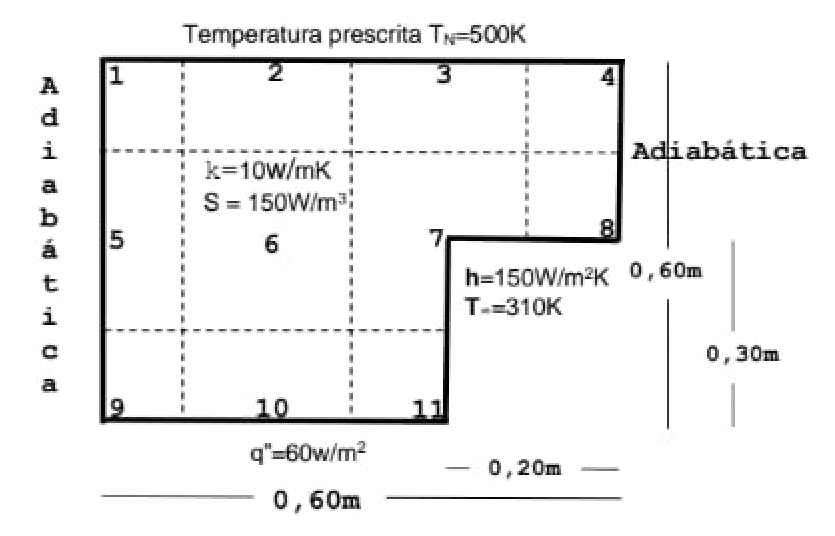
\includegraphics[scale=0.60]{problemaED05.png}
\end{figure}

Em regime permanente, o processo de condução na Figura \ref{fig:problemaplaca} possui 
equação dada por 

\begin{equation}\label{eq:pdecomplete}
    \frac{\partial}{\partial{x}} \left(k\frac{\partial{T}}{\partial{x}}\right) +
    \frac{\partial}{\partial{y}} \left(k\frac{\partial{T}}{\partial{y}}\right) +
    S = 0
\end{equation}

Em que o domínio de solução da equação diferencial parcial de \eqref{eq:pdecomplete} é

\begin{equation}\label{eq:domain}
    0 < x < 0,6 \un{m} \quad , \quad 0 < y < 0,6 \un{m}
\end{equation}

E as condições de contorno são:

\begin{itemize}
    \item Fronteira oeste: como é adiabática, temos $\diff{T}{x} = 0$;
    \item Fronteira norte: como temos tempeartura prescrita, temos $T(y=0,6) = 500 \un{K}$ ;
    \item Fronteira sul: como temos fluxo prescrito, temos, pela Lei de Fourier, $-k\diff{T}{y} = 60 \un{W/m$^2$}$
    \item Fronteira leste, parte inferior $x = 0,4 \un{m}$ e $0 < y < 0,3 \un{m}$, temos conveccção: $-k\diff{T}{x} = h\left(T(x=0,4) - T_{\infty}\right)$;
    \item Fronteira leste, parte superior $x = 0,6 \un{m}$ e $0,3 < y < 0,6 \un{m}$, temos adiabática: $\diff{T}{x} = 0$;
    \item Fronteira leste, parte deitada $y = 0,3 \un{m}$ e $0,4 < x < 0,6 \un{m}$, temos conveccção: $-k\diff{T}{y} = h\left(T(y=0,3) - T_{\infty}\right)$;
\end{itemize}

\end{document}
